\documentclass[../main.tex]{subfiles}


\begin{document}

\section{Approach}

Our approach is constructed as follows:

First is method declaration. We used AST Parser Tool to catch each method and get the information, which means, the \textit{startLineNumber, endLineNumber, methodName, methodParameters, methodType, methodBody}. This costs extra time and can be improved in future work.

Second is the tokenization of method body and get the frequency of each token, which includes the comment and white space removal process.

Third, for each method, we have a list of tokens, these tokens fall into 9 categories: \textit{methodParameter, methodType, tokenListNumber, tokenListType, tokenListKeyword, tokenListMarker, tokenListOperator, tokenListOther1, tokenListOther2}. The purpose of doing so is that these categories have different weights, for example, two pieces of code both have 2 type names: ``int'', that provides no useful information, however, if two pieces of code both have 2 method parameter names: ``drawVerticalLine'', that means these pair are more likely the same.

A list of categorized tokens are shown in table \ref{tab:Table_1}:\\

\begin{tablehere}
\footnotesize
\begin{tabular}[h]{|c|c|c||c|c|c|}
\hline
Token & Category & Freq 	& Token & Category & Freq\\
\hline
int & Type &1 		&  ) & Marker & 6\\
\hline
for & Keyword & 1 	& \} & Marker & 2\\
\hline
i & Other1 & 8		& \{ & Marker & 1\\
\hline
System & Other1 & 3	& + & Operator & 6\\
\hline
out & Other1 & 3	& = & Operator & 1\\
\hline
println & Other1 & 3	& - & Operator & 1\\
\hline
toBinary & Other1 & 1	& < & Operator & 1\\
\hline
Integer & Other1 & 1	& : & Other2 & 2\\
\hline
toBinaryString & Other1 & 1	& 5.0 & Num & 1\\
\hline
( & Marker & 6		& 33.0 & Num & 1\\
\hline
\end{tabular}\\
\caption{A List of Token Frequency}\label{tab:Table_1}
\end{tablehere}

Fourth, similarity of \textit{methodParameter} is caculated with bigram similarity. If ``drawVerticalLine'' and ``VerticalDrawLine'' appear in two code fragments respectively, we don't want to take them as different. So two similar variable names will be compared by bigram similarity, if they are similar, they will be taken as the same and their frequencies will be compared later.

Fifth, after the pretreatment of variable names, a similarity algorithm is applied to each category, and the number of similarity will be caculated, so we have 9 similarity numbers.

Finally, the 9 similarity numbers are given different weights and the final similarity will be calculated. A threshold is introduced, if the similarity is higher than the threshold, the result will be printed out: clone group number, similarity number, method name 1, start and end line number, method name 2, start and end line number.

A diagram describing the whole process is shown in Fig:\ref{fig:Graph_1}.\\

\begin{figurehere}
\centering 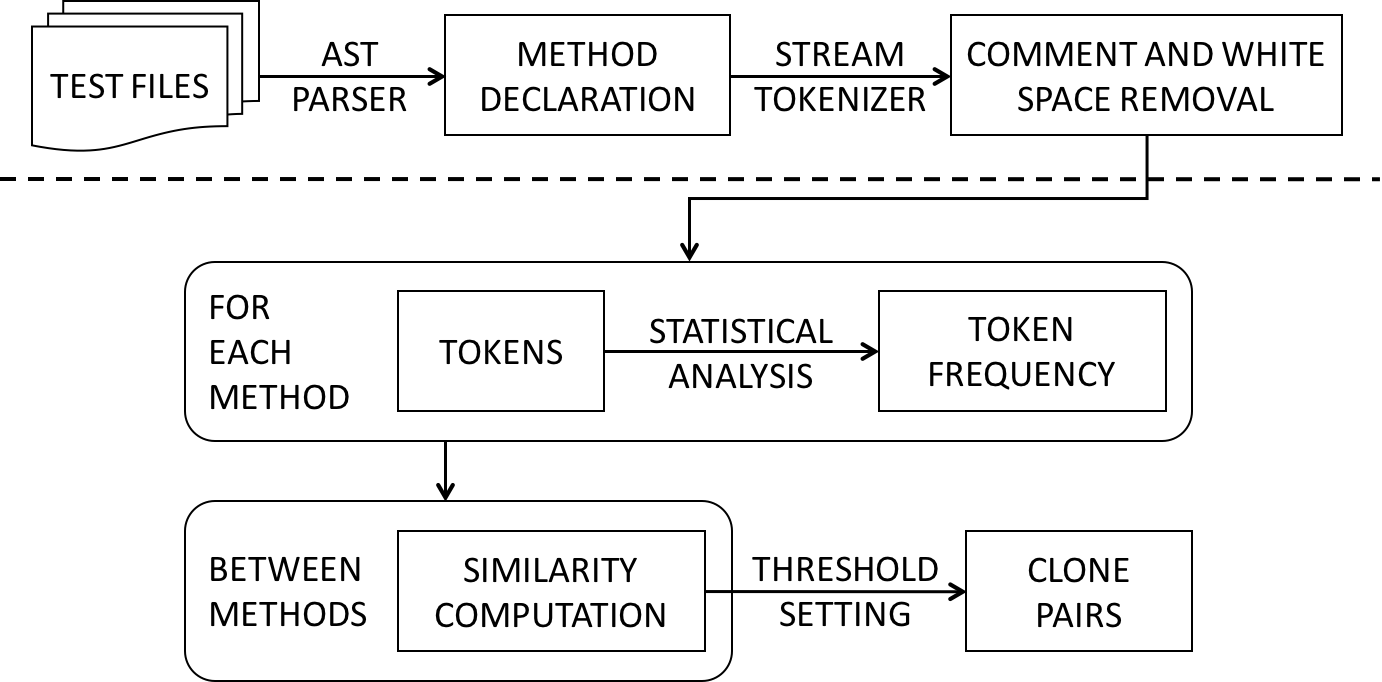
\includegraphics[width = 0.45 \textwidth]{Graph_1} 
\caption{Overall Project Framework} \label{fig:Graph_1}
\end{figurehere}

During the final step, different weights are given to different categories, however, picking 9 weights arbitrarily may not be resonable. So we used Machine Learning method to set the weights. Provided training files with ``ground truth'', machine learning process will decide the most proper weights, which is much more resonable than setting by hand. After actual testing, it turns out machine learning does provide a better result.\\

\begin{figurehere}
\centering 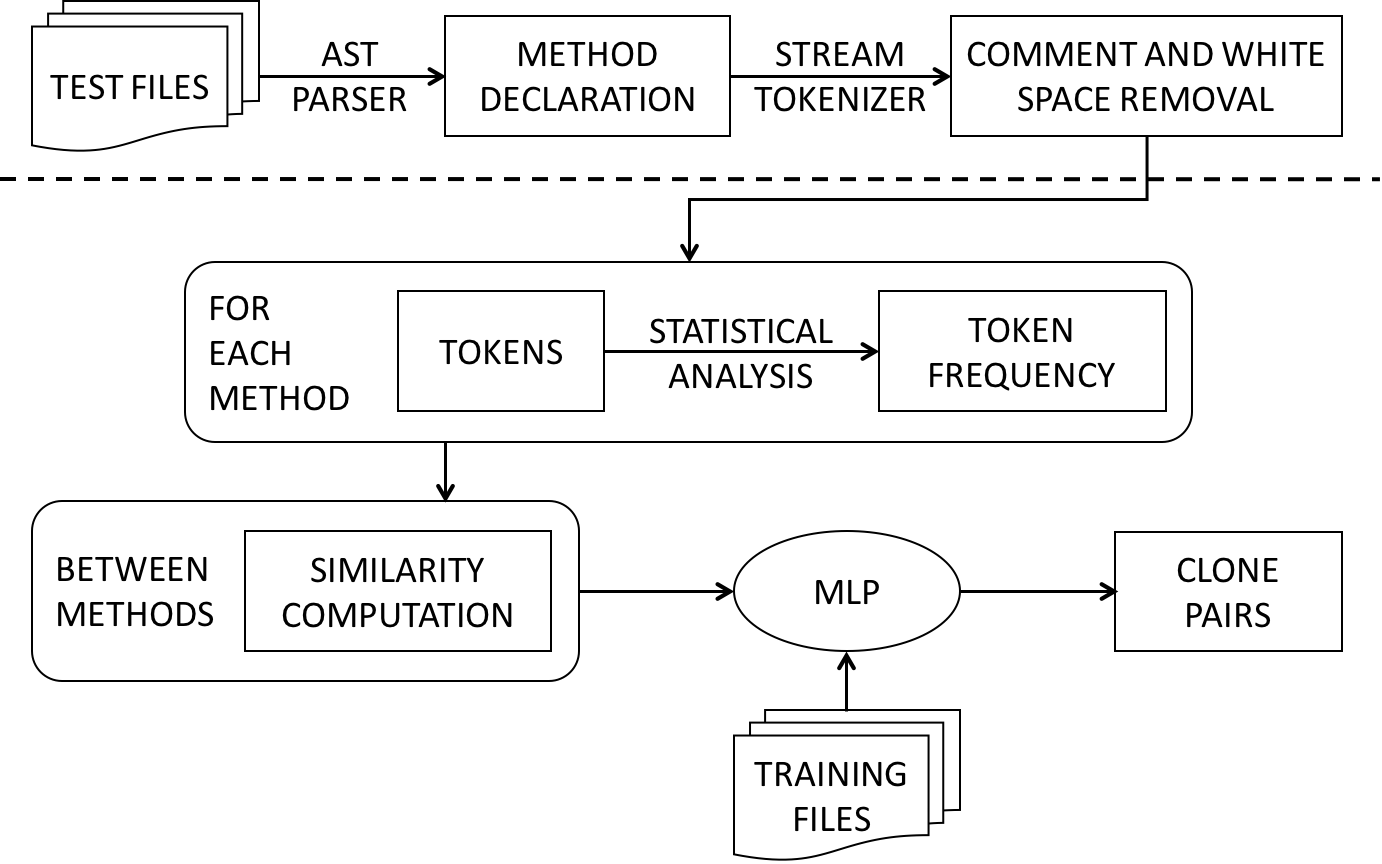
\includegraphics[width = 0.45 \textwidth]{Graph_2} 
\caption{Project Framework with Machine Learning} \label{fig:Graph_2}
\end{figurehere}

\end{document}